\documentclass[12pt,a4paper]{report}
\usepackage[utf8]{inputenc}
\usepackage[top=1.5cm,bottom=1cm,right=1cm,left=1cm]{geometry}
\usepackage{amsmath,amsfonts,amssymb,mathrsfs,tikz}
\pagestyle{empty}
\usetikzlibrary{backgrounds,shadings,calc}
\colorlet{fff}{blue!30!green!40}
\colorlet{ggg}{fff!80!black}
\tikzstyle{a}=[draw=ggg,right color=ggg,left color=ggg!50!black]
\tikzstyle{b}=[draw=ggg,right color=fff,left color=fff!25]
\newdimen\bv 
\bv=1.5cm
\def\titlebox#1{%
\begin{tikzpicture}
\node[minimum width=0.75\linewidth,align=center,font=\bfseries\huge] (1) {#1};
\begin{scope}[on background layer]
\coordinate (a) at($(1.south east)+(-.25\bv,-.25\bv)$);
\coordinate (b) at($(a)+(.5\bv,0)$);
\coordinate (e) at($(1.south west)+(.25\bv,.25\bv)$);
\coordinate (d) at($(1.north west)+(0,.25\bv)$);
\coordinate (c) at($(d)+(.25\bv,0)$);
\coordinate (f) at($(d)+(-.25\bv,0)$);
\path [draw=ggg,right color=fff,left color=fff,middle color=white](f)arc(180:270:.25\bv)--(1.north east)arc(90:0:.25\bv)--(b)arc(0:90:.25\bv)--(1.south west)arc(-90:-180:.25\bv)--cycle;
\path [a] (d)-|(e)arc(0:-180:.125\bv)--cycle;
\path [b](c)--(e)arc(0:180:.25\bv)--(f)arc(180:0:.25\bv)--cycle;
\path [b](a)|-(1.south east)--+(0,-.25\bv)arc(0:180:.125\bv)--cycle;
\path[a](1.south east)arc(90:-180:.25\bv)arc(180:0:.125\bv)--cycle;
\end{scope}
\end{tikzpicture}
}
\def\shape#1{\scalebox{#1}{%
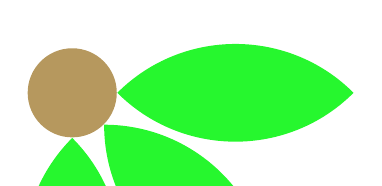
\begin{tikzpicture}
\node[circle,fill=brown!75!fff,inner sep=4mm](5){};
\foreach \i in {0,1,2}{
\fill[green!75!fff,transform canvas={rotate=-\i*45}](5.east)to[bend left=45]+(3,0)to[bend left=45]cycle;
}
\end{tikzpicture}
}}

\def\size{1}
\parindent=0mm
\begin{document}
\begin{tikzpicture}[remember picture,overlay]
\coordinate(1)at ([shift={(225:\size)}]current page.north east);
\coordinate(2)at ([shift={(-45:\size)}]current page.north west);
\coordinate(3)at ([shift={(45:\size)}]current page.south west);
\coordinate(4)at ([shift={(135:\size)}]current page.south east);
\foreach \i in {0,1,...,60}{\foreach \j/\k in {1/4,2/3}{
\path(\j)--node[pos=\i/60]{\shape{0.1}}(\k);
}}
\foreach \i in {1,2,...,45}{\foreach \j/\k in {1/2,4/3}{
\path(\j)--node[pos=\i/45]{\shape{0.1}}(\k);
}}
\end{tikzpicture}
\null
\hfill
\begin{minipage}[t]{0.2\linewidth}
\vglue-.5\baselineskip
\includegraphics[width=\linewidth,height=3cm]{example-image-a}
\end{minipage}\hfill
\begin{minipage}[t]{0.48\linewidth}
\centering\bfseries\slshape
République Algérienne Démocratique et Populaire\\
Ministère de l'enseignement supérieur et de la recherche scientifique\\

\end{minipage}\hfill
\begin{minipage}[t]{0.2\linewidth}
\vglue-.5\baselineskip
\includegraphics[width=\linewidth,height=3cm]{example-image-b}
\end{minipage}
\hfill
\null\vglue5mm
\uppercase{\bfseries%
Université Mohamed El Bachir El Ibrahimi - BBA-
}
\centering\vglue3cm\sl
\underline{\bf\Large MEMOIRE DE MASTER}
\vglue5mm
\begin{center}
\underline{\slshape\bfseries Thème}
\vskip3mm
\titlebox{%
type your title here\\........\\.......
}
\end{center}
\vglue5mm
\begin{minipage}[t]{8cm}
\underline{\bf Présenté par:}\\[3mm]\bf
Nom et prénom
\end{minipage}
\hfill
\begin{minipage}[t]{5cm}
\underline{\bf Enquadré par:}\\[3mm]\bf
\hfill Nom \& Prénoms
\end{minipage}
\vfill
\centering\bf
Promotion: mois \& année
\end{document}